% ============================ Enrico Ribiani 16-03-2021 ====================================================================
% Base per i documenti  
\documentclass[12pt]{article}
% ------------ pacchetti necessari ----------------
\usepackage[a4paper, total={6in, 8in},margin=1in]{geometry} % formattazione decente della pagina
\usepackage{graphicx}                            % need for figure
\usepackage{amsmath}
\usepackage{amsfonts}                            % if you want the fonts
\usepackage{amssymb}                             % if you want extra symbols
\usepackage{graphicx}  
\renewcommand{\figurename}{Figura}  
\renewcommand{\contentsname}{Indice}                        % need for figures
\usepackage{mathptmx}
\usepackage{float}                               % serve per mettere tabelle e immagini dove si vuole 
\usepackage[utf8]{inputenc}
\usepackage{textcomp}
\usepackage[hang,flushmargin,bottom]{footmisc}   % footnote format
\usepackage{fancyhdr, lastpage}
\usepackage{titlesec}
\usepackage[table,dvipsnames]{xcolor}
%\pagestyle{fancy}
%\renewcommand{\headrulewidth}{0pt}
%\renewcommand*\contentsname{Indice}
\titleformat{\section}{\normalsize\bfseries}{\thesection.}{1em}{}	% required for heading numbering style
\titleformat*{\section}{\Large\bfseries}
\titleformat*{\subsection}{\large\bfseries}
%\usepackage{siunitx}
%\usepackage{tikz}
\usepackage{circuitikz}
\usepackage{multicol}
%\usepackage[siunitx]{circuitikz}
\usepackage{multirow}
\usepackage{tikz}
\usepackage{amsmath}
\usetikzlibrary{angles,quotes}
\usepackage{placeins}

\usepackage{wasysym}
%===================links=================
\usepackage{hyperref}
\hypersetup{
    colorlinks=true,
    linkcolor=darkgray,
    filecolor=Green,      
    urlcolor=Cyan,
    pdftitle={SAMPLE},
    pdfpagemode=FullScreen,
    }
%===================inizio pagina del titolo=================
\begin{document}
\begin{titlepage}
	\begin{center}
		% ------------------ inizio immagine logo ----------
		\begin{figure}
			\centering
			
\includegraphics[scale=1.3]{/home/r1bbi/Documenti/latec/logo.png}

		\end{figure}
		% ------------------ fine immagine logo ----------
		% ------------------ fine immagine logo ----------
		-------------------------------------------------------------------------------------\\
		\vspace{2\baselineskip}
		\large Prova n°5
		\hfill
		\large $5^a$   AUB\\
		\begin{flushleft}
			\large Enrico Ribiani\\
			\large Daniel Graziadei\\
			\large Gruppo 11\\
		\end{flushleft}


		\vfill

		\Huge{\textbf{Raddrizzatore monofase a semionda su carico ohmico-induttivo }}\\
		\vfill
		\vfill
		\large{9-3-2023}
	\end{center}
	%=============== fine pagina titolo ===============
\end{titlepage}
\thispagestyle{empty}
\tableofcontents
\newpage
\setcounter{page}{1}
\vskip 1cm
\section{Scopo}
Verificare il comportamento qualitativo in modo sperimentale delle tensioni  e correnti in
ingresso e uscita da un raddrizzatore ohmico-induttivo.\\

\section{Schema}
\begin{figure}[!h]
	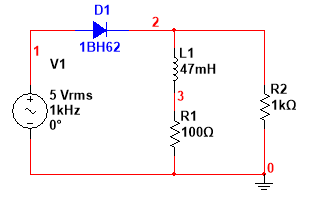
\includegraphics[scale=0.7]{schema.PNG}
\end{figure}

\section{Materiale e Strumenti}
\begin{multicols}{2}
	\begin{itemize}
		\item Generatore AC 5V
		\item diodo 1BH62
		\item Resistenza da $100\Omega$
		\item Resistenza da $1k\Omega$
		\item Induttore 47mH
	\end{itemize}
	\vfill\null
	\columnbreak
	\begin{itemize}
		\item Oscilloscopio
	\end{itemize}
	\vfill\null
\end{multicols}

\section{Contenuti Teorici}
L'induttore ha lo scopo di assorbire energia nel momento in cui sia tensione che corrente sono entrambi
positivi.\\ Tale energia è restituita quando la tensione si inverte, questo permette la circolazione della
corrente anche quando la semionda di tensione dell'alimentazione diventa negativa. \\
Così L'andamento della tensione ai capi del carico assume l'andamento V2 (transient).
Quando la corrente I1 si abbassa, la V2 diventerà negativa.\\
\section{Raccolta dei dati}
\begin{figure}[H]
	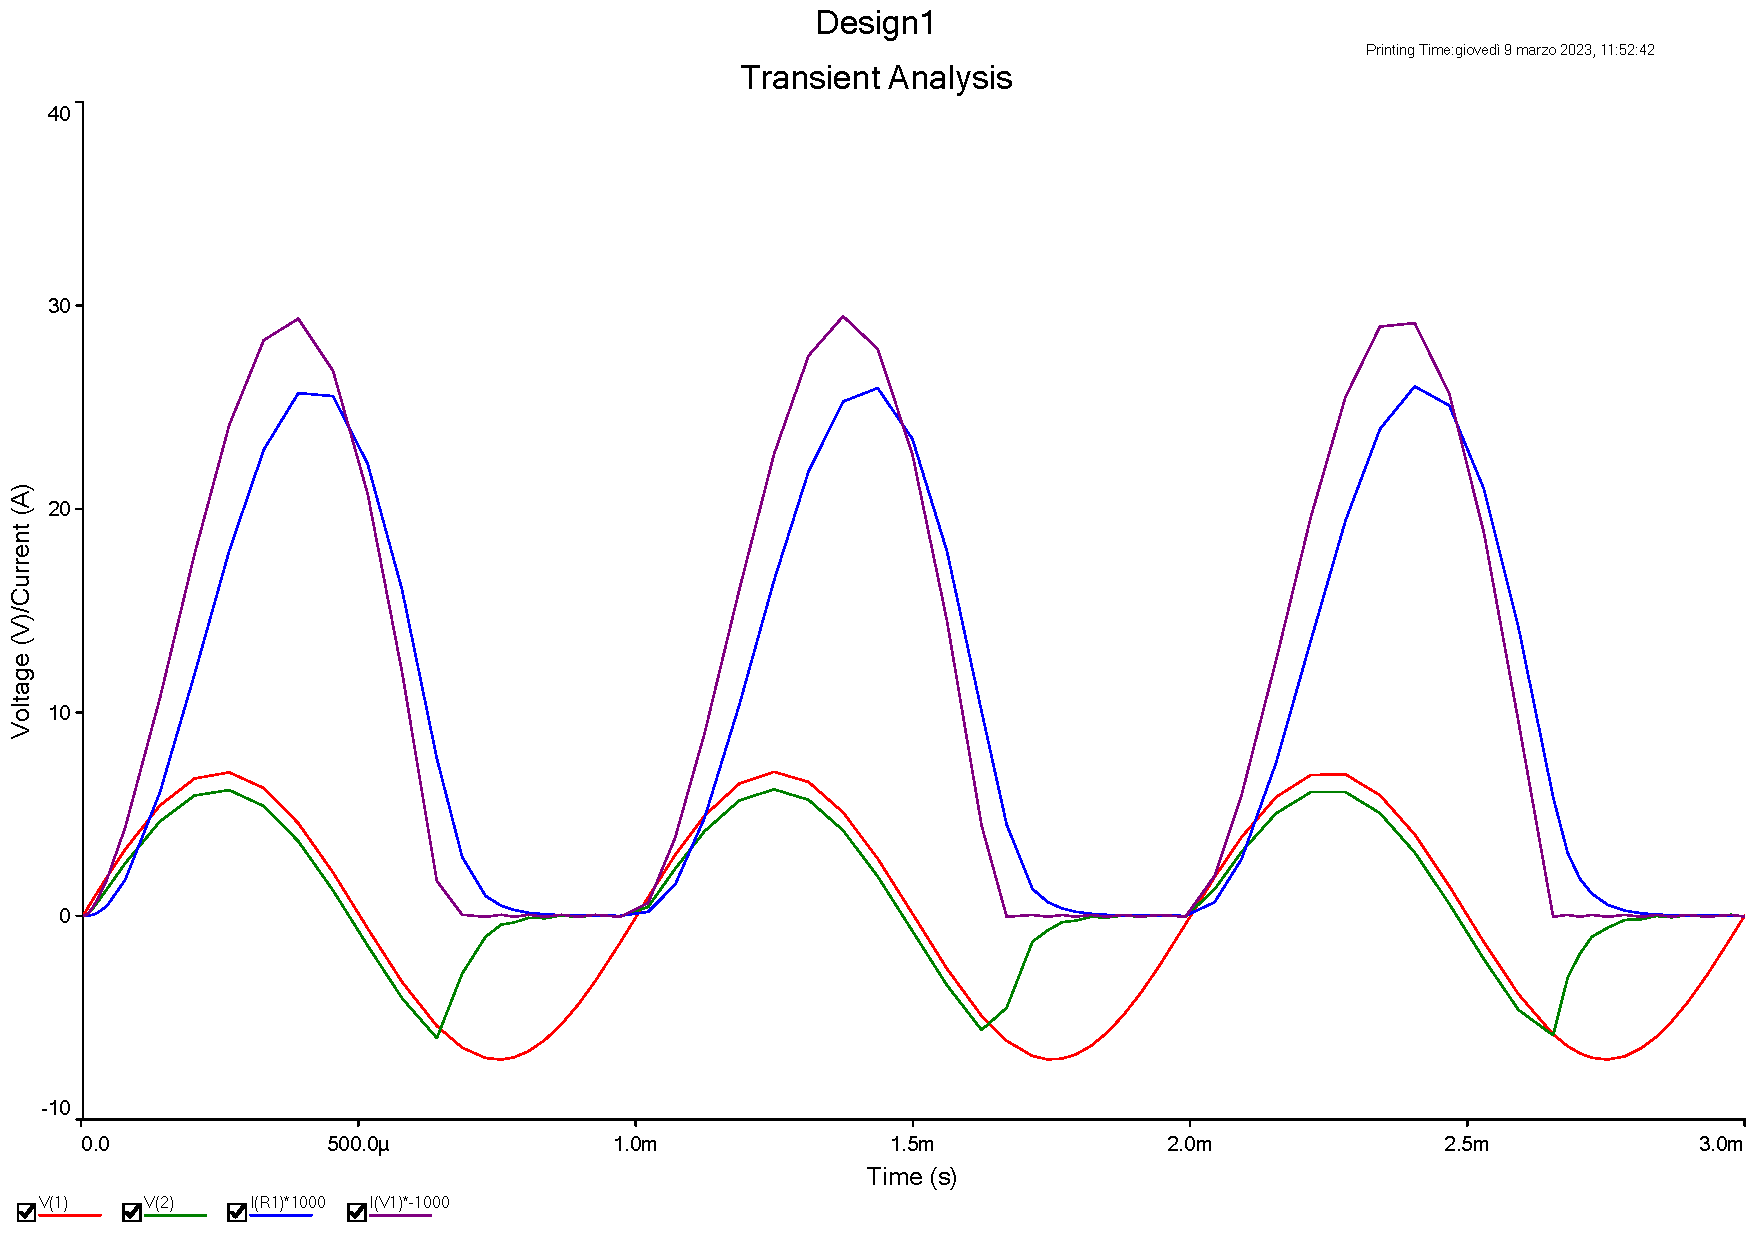
\includegraphics[scale=0.5]{osc.pdf}
\end{figure}

\section{Calcoli}
$I_{1}=\frac{V_{1}}{R1}$
\section{Analisi critica dei risultati e conclusioni}
Lo scopo è verificato poichè dal grafico riportato possiamo notare che il circuito si comporta come previsto dai
contenuti teorici, infatti possiamo notare che la corrente in uscita (in blu) è sfasata rispetto a quella in ingresso
(in viola) e ha anche un'ampiezza minore poichè per colpa della magnetizzazione dell'induttore non segue perfettamente
la tensione.\\\
Osserviamo che la tensione sul carico (in verde)  oltre ad avere un'ampiezza ridotta presenta un picco negativo coincidente
con la fase di smagnetizzazione dell'induttore.\\
\end{document}


